% Choose one to switch between slides and handout
%\documentclass[]{beamer}
\documentclass[handout]{beamer}

% Video Meta Data
\title{Bitcoin, Blockchain and Cryptoassets}
\subtitle{Blockchain Forks}
\author{Prof. Dr. Fabian Schär}
\institute{University of Basel}

% Config File
% Packages
\usepackage[utf8]{inputenc} 
\usepackage{hyperref}
\usepackage{gitinfo2}
\usepackage{tikz}
\usepackage{amsmath}
\usepackage{bibentry}
\usepackage{xcolor}
\usepackage{caption}

% Beamer Template Options
\beamertemplatenavigationsymbolsempty
\setbeamertemplate{footline}[frame number]
\setbeamercolor{structure}{fg=black}
\setbeamercolor{footline}{fg=black}
\setbeamercolor{title}{fg=black}
\setbeamercolor{frametitle}{fg=black}
\setbeamercolor{item}{fg=black}
\setbeamercolor{}{fg=black}
\setbeamercolor{bibliography item}{fg=black}
\setbeamercolor*{bibliography entry title}{fg=black}
\setbeamertemplate{items}[square]
\setbeamertemplate{enumerate items}[default]
\captionsetup[figure]{labelfont={color=black},font={color=black}}
\captionsetup[table]{labelfont={color=black},font={color=black}}

\setbeamertemplate{bibliography item}{\insertbiblabel}

% Link Icon Command
\newcommand{\link}{%
    \tikz[x=1.2ex, y=1.2ex, baseline=-0.05ex]{% 
        \begin{scope}[x=1ex, y=1ex]
            \clip (-0.1,-0.1) 
                --++ (-0, 1.2) 
                --++ (0.6, 0) 
                --++ (0, -0.6) 
                --++ (0.6, 0) 
                --++ (0, -1);
            \path[draw, 
                line width = 0.5, 
                rounded corners=0.5] 
                (0,0) rectangle (1,1);
        \end{scope}
        \path[draw, line width = 0.5] (0.5, 0.5) 
            -- (1, 1);
        \path[draw, line width = 0.5] (0.6, 1) 
            -- (1, 1) -- (1, 0.6);
        }
    }

% Custom Titlepage
\defbeamertemplate*{title page}{customized}[1][]
{
  \vspace{-0cm}\hfill\includegraphics[width=2.5cm]{../config/logo_cif} 
  \includegraphics[width=1.9cm]{../config/seal_wwz} 
  \\ \vspace{2em}
  \usebeamerfont{title}\textbf{\inserttitle}\par
  \usebeamerfont{title}\usebeamercolor[fg]{title}\insertsubtitle\par  \vspace{1.5em}
  \small\usebeamerfont{author}\insertauthor\par
  \usebeamerfont{author}\insertinstitute\par \vspace{2em}
  \usebeamercolor[fg]{titlegraphic}\inserttitlegraphic
    \tiny \noindent \texttt{Commit Hash: \gitHash}\\ 
	\texttt{Commit Time: \gitAuthorIsoDate}\\ \vspace{1em}
  \link \href{https://github.com/cifunibas/Bitcoin-Blockchain-Cryptoassets/blob/main/slides/intro.pdf}
  {Get most recent version}\\
  \link \href{https://github.com/cifunibas/Bitcoin-Blockchain-Cryptoassets/blob/main/slides/intro.pdf}
  {Watch video lecture}\\ \vspace{1em}
  License: \texttt{Creative Commons Attribution-NonCommercial-ShareAlike 4.0 International}\\\vspace{2em}
  \includegraphics[width = 1.2cm]{../config/license}
}


%%%%%%%%%%%%%%%%%%%%%%%%%%%%%%%%%%%%%%%%%%%%%%
%%%%%%%%%%%%%%%%%%%%%%%%%%%%%%%%%%%%%%%%%%%%%%
\begin{document}

\thispagestyle{empty}
\begin{frame}[noframenumbering]
	\titlepage
\end{frame}

%%%


\begin{frame}{Greatest Accumulated Difficulty}
	There is a simple rule to identify the most recent state of the ledger:
	\vspace{1em}
	
	\begin{description}
		\item[\textbf{Intuition:}] The longest chain, i.e., the chain with the longest sequence of valid blocks is seen as the most recent version.
		\item[\textbf{Rule:}] The chain with the \color{focus} greatest accumulated difficulty \color{black} is seen as the most recent version. 
	\end{description}
	
	\vspace{1em}
	
	Under normal circumstance this rule leads to a clear status quo. Forks are the exception\dots
\end{frame}


%%%
\begin{frame}{What is a Fork?}

\color{focus} Disagreement on the current state \color{black} of the ledger that leads to two or more competing versions of the blockchain.

\begin{figure}[h]
  	\center
  	\resizebox{0.55\textwidth}{!}{
	\input{../assets/figures/simple-fork.tex}
	}
\end{figure}

\vspace{1em}
\textbf{Forks may arise for two distinct reasons:}
\begin{enumerate}
	\item Same rules ($A = B$): Process-based, i.e., agents have not the same information set or choose to compete.
	\item Different rules ($A \neq B$): Protocol-based, i.e., agents have a different understanding of consensus rules.
\end{enumerate}

\end{frame}
%%%

%%%
\begin{frame}{Classification of Forks}

\footnotesize
\begin{table}
  \center
  \begin{tabular}[]{rll}
    \hline\hline 
    ~	& \textbf{Process-based} & \textbf{Protocol-based}      \\
    ~	& $(A=B=S)$ & $(A \neq B)$ \\\cline{2-3} 
    \rule{0pt}{3ex}    
    \textbf{Unintentional} & Probabilistic Block Race & Client Incompatibility \\ 
        &  & \makecell[l]{\hspace{1em}\textbullet{ }\footnotesize{Soft Fork} \\   \hspace{1em}\textbullet{ }\footnotesize{Hard Fork} \\  \hspace{1em}\textbullet{ }\footnotesize{Forced Fork} }   \\
    \rule{0pt}{3ex}    
    \textbf{Deliberate}    & Block Withholding \&  & Rule Change                  \\
        & \makecell[l]{Forced Block Race\vspace{2.5em}} & \makecell[l]{\hspace{1em}\textbullet{ }\footnotesize{Soft Fork} \\   \hspace{1em}\textbullet{ }\footnotesize{Hard Fork} \\  \hspace{1em}\textbullet{ }\footnotesize{Forced Fork} }     \\
    \hline\hline
  \end{tabular}
  \caption{The four fork types \cite{schar2020blockchain}}
  \label{tbl:classification}
\end{table}
	
\end{frame}
%%%	

%%%
\begin{frame}{Process-based Forks}

\textbf{Probabilistic block race:} Block creation is probabilistic. Two or more blocks may be created at approx. the same time.
\vspace{1.5em}	

\uncover<2->{
\textbf{Forced block race:} Deliberate mining of own chain with the goal to overtake consensus version.
\vspace{1.5em}	


\textbf{Block withholding:} Purposeful delay of propagation of own valid candidate block to gain head start on next block.\cite{eyal2014majority}
\vspace{1.5em}	
}

\uncover<3->{
$\Rightarrow$ All temporary and resolved through accumulated difficulty (longest chain rule).
}
	
\end{frame}
%%%

%%%
\begin{frame}{Protocol-based forks}

\textbf{Client incompatibility:} Delta in consensus rule implementations by different network client software, causing some nodes to accept certain blocks rejected by others. Root causes:
\begin{itemize}
	\item Loosely defined consensus rules
	\item Software bugs
\end{itemize}
\vspace{0.5em}
Example: Upgrade to Bitcoin client 0.8 in 2013
\vspace{1em}	

\uncover<2->{
\textbf{Rule change:} Part of the network decides to alter the consensus rule set $S$ and proceed with adapted protocol.
\vspace{0.5em}

Example: Split of Bitcoin ABC over Blocksize increase.
\vspace{2em}	
	
}

\uncover<3->{
$\Rightarrow$ Not resolved automatically and may cause permanent splits. Let us denote the old rules and the new rules by $S_{old}$ and $S_{new}$ respectively and analyze various situations.
}
	
\end{frame}
%%%

%%%
\begin{frame}{Types of Protocol-based Forks}


\begin{columns}[T]
	\begin{column}{0.3\textwidth}
		\center		
		\textbf{Soft Fork}\\
		\vspace{0.5em}
		\begin{figure}[h]
  			\resizebox{0.9\textwidth}{!}{
			%%% Figure from: Schär, Fabian. "Blockchain Forks: A Formal Classification Framework and Persistency Analysis." (2020).

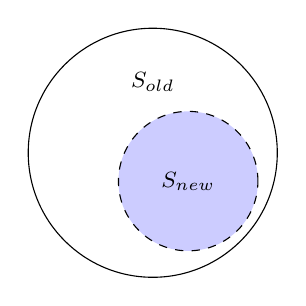
\begin{tikzpicture}[domain=0:8,scale=0.9, every node/.style={scale=1}]
  \filldraw[draw=black,fill=white] (0,0) circle (50pt) node[below=-1.15cm,color=black]{\footnotesize{$S_{old}$}};
  \filldraw[draw=black,fill=blue!20,dashed] (0.5,-0.4) circle (28pt) node[color=black]{\footnotesize{$S_{new}$}};
\end{tikzpicture}

			}
		\end{figure}
		\vspace{1em}
		$S_{new}\subset S_{old}$
	\end{column}
	\begin{column}{0.3\textwidth}
		\center
 		\textbf{Hard Fork}\\
 		\vspace{1em}
 		\begin{figure}[h]
  			\center
  			\resizebox{0.9\textwidth}{!}{
			\input{../assets/figures/hard-fork.tex}
			}
		\end{figure}
 		\vspace{1.5em}
 		$S_{new}\supset S_{old}$
	\end{column}
		\begin{column}{0.3\textwidth}
		\center
 		\textbf{Forced Fork}\\
 		\vspace{0.5em}
 		\begin{figure}[h]
  			\center
  			\resizebox{0.9\textwidth}{!}{
			%%% Figure from: Schär, Fabian. "Blockchain Forks: A Formal Classification Framework and Persistency Analysis." (2020).

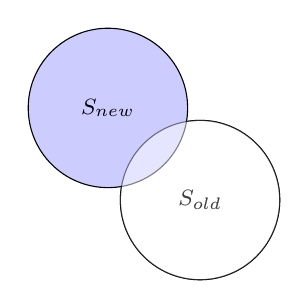
\begin{tikzpicture}[domain=0:8,scale=0.9, every node/.style={scale=1}]
  \filldraw[draw=black, fill=white] (0.9,-0.9) circle (32pt) node[color=black]{\footnotesize{$S_{old}$}};
  \filldraw[draw=black,fill=blue!20] (-0.4,0.4) circle (32pt) node[color=black]{\footnotesize{$S_{new}$}};
  \filldraw[draw=black, fill=white, opacity=0.5] (0.9,-0.9) circle (32pt) node[color=black]{\footnotesize{$S_{old}$}};
\end{tikzpicture}

			}
		\end{figure}
		\vspace{0.8em}
 		$(S_{new}\setminus S_{old} \neq \emptyset)$\\$\wedge$\\ $(S_{old}\setminus S_{new} \neq \emptyset)$
	\end{column}
\end{columns}

\vspace{0.5em}

\begin{center}
	Figure: Types of protocol-based forks \cite{schar2020blockchain}
\end{center}

	
\end{frame}
%%%

%%%
\begin{frame}{Fork Persistency by Type and Dominance Scenario}

	\begin{table}
		\input{../assets/figures/fork-types.tex}
		\caption{Persistency by fork type and scenario \cite{schar2020blockchain}}
		\label{tbl:forkpersistencies}
	\end{table}

	


	
\end{frame}
%%%



%%%
\begin{frame}{Why Should We Care about Forks?}


\begin{enumerate}
	\item \textbf{Uncertainty:} Confirmation status of transactions.
	\item \textbf{Confusion:} Various competing versions of the asset.
	\item \textbf{Security Tokens:} Competing promises delivery of 1 good.
	\item \textbf{Cost driver:} Tax / legal questions, maintaining compatibility.
\end{enumerate}

\vspace{1em}
\color{focus} \textbf{But:} \color{black} Risk of fork may increase stability and strengthen status quo.

	
\end{frame}
%%%	

%%%
\begin{frame}%[allowframebreaks]
\frametitle{References and Recommended Reading}

	\bibliographystyle{amsplain}
	\bibliography{../assets/bib/refs}

\end{frame}


\end{document}